%%%%%%%%%%%%%%%%%%%%%%%%%%%%%%%%%%%%%%%%%%%%%%%%%%%%%%%%%%%%%%%%%%%%%%%%%%%%%%%%
%2345678901234567890123456789012345678901234567890123456789012345678901234567890
%        1         2         3         4         5         6         7         8

% \documentclass[letterpaper, 10 pt, conference]{ieeeconf}  % Comment this line out if you need a4paper

\documentclass[a4paper, 11.5pt, conference]{ieeeconf}      % Use this line for a4 paper

\IEEEoverridecommandlockouts                              % This command is only needed if 
                                                          % you want to use the \thanks command

\overrideIEEEmargins                                      % Needed to meet printer requirements.

%In case you encounter the following error:
%Error 1010 The PDF file may be corrupt (unable to open PDF file) OR
%Error 1000 An error occurred while parsing a contents stream. Unable to analyze the PDF file.
%This is a known problem with pdfLaTeX conversion filter. The file cannot be opened with acrobat reader
%Please use one of the alternatives below to circumvent this error by uncommenting one or the other
%\pdfobjcompresslevel=0
%\pdfminorversion=4

% See the \addtolength command later in the file to balance the column lengths
% on the last page of the document

% The following packages can be found on http:\\www.ctan.org
\usepackage{graphics}
%\usepackage{parskip} % for pdf, bitmapped graphics files
%\usepackage{epsfig} % for postscript graphics files
\usepackage{mathptmx} % assumes new font selection scheme installed
\usepackage{times} % assumes new font selection scheme installed
\usepackage{amsmath} % assumes amsmath package installed
\usepackage{amssymb}  % assumes amsmath package installed
\usepackage{float}
\usepackage{subcaption}
\usepackage{caption}
\usepackage{hyperref}
\hypersetup{hidelinks}
\title{\LARGE \bf Collision Monitoring for a Mobile Manipulator Based on Biologically-Inspired Dynamical Systems for Movement Generation}
\usepackage[colorinlistoftodos]{todonotes}

\author{Sreenivasa Hikkal Venugopala, Zain Ul Haq, and Urvashi Negi \\ {\small \textbf{Advisor:} Djordje Vukcevic}}
\setlength{\parskip}{0pt}

\begin{document}



\maketitle
\thispagestyle{empty}
\pagestyle{empty}


%%%%%%%%%%%%%%%%%%%%%%%%%%%%%%%%%%%%%%%%%%%%%%%%%%%%%%%%%%%%%%%%%%%%%%%%%%%%%%%%
\begin{abstract}
The computations involving the robotic manipulators, that is robotic arms and the mobile manipulators, that is mobile base (robot base) up until recent times are limited in the degree of operation and have several restrictions due to rigid movements, the control algorithms for these manipulators are usually complex involving various operations such as planning, perception, and so on. This makes the computations complex and time consuming and make it hard for its usage in the dynamic environments involving other robots, humans. To overcome these issues, in this research work, we propose to extend the implementation of the control algorithms which is implemented based on collision monitoring \cite{Khatib} and collision avoidance \cite{Hoffmann} for controlling the movements of the robotic arms from colliding with each other and to extend it to avoid collision with the mobile base as well. Along with this, we also implement the control algorithms for mobile base that helps in monitoring and avoiding the collision with any obstacles and helps in safe maneuvering towards the goal.

\end{abstract}


%%%%%%%%%%%%%%%%%%%%%%%%%%%%%%%%%%%%%%%%%%%%%%%%%%%%%%%%%%%%%%%%%%%%%%%%%%%%%%%%
\section{Introduction} 

%Background ---------------
The robotic arms or the robotic manipulators are used in various applications ranging from industrial applications to domestic applications. They are widely used in industrial applications such as to support human in the production lines of heavy machineries for the purpose of assembling spare parts, welding, painting and so on, and in domestic applications such as robotic prosthetics, robotic assistants, and so on. Along with these applications, A robot as a whole, that is including both arms and the mobile base, poses useful in various applications such as warehouse management. All these applications require more robust and highly adaptable software and hardware components. For increasing the efficiency and the robustness of the functioning of the robotic manipulators in industrial applications, a precomputed trajectories will be provided \cite{Hoffmann}, but these precomputed trajectories will not consider the dynamic movement of human and other obstacles. On the other hand, various operators are used to control the movement and functioning of the robotic prosthetics, but this does not provide free flow motion for the arms or prosthetics. On contrary it takes a lot of time and effort to train the robotic manipulators to perform a safe and free flow movement, but this is a high cost solution which is not weighable in all scenarios.

One of the solution approach to handle the control algorithm problem is to make use of the dynamic movement primitives, these are generated during the movement of the robot manipulators resulting in real-time collision monitoring and avoidance. There were many approaches proposed as a solution to this problem, based on the approaches proposed by \cite{Hoffmann} and \cite{Khatib} a library named `Implementation of biologically-inspired dynamical systems for
movement generation: automatic real-time goal adaptation and obstacle avoidance \cite{sdpss20}' was developed (\url{https://github.com/HBRS-SDP/sdp\_ss20\_collision\_monitoring\_for\_robotic\_manipulators}). This library handles the collision monitoring and collision avoidance for robotic arms in real-time and it incorporates the idea of dynamic movement primitives and the potential field method for active collision monitoring and avoidance. Here the dynamic primitives and the obstacles are considered as the basic primitives having shape and volume. The obstacle is avoided by planning a trajectory in such a way that a steering angle is computed in a potential field which steers the arms away from the obstacle and then converge towards the goal.

In this work, we propose to implement and extend the previous work by formulating the mobile manipulator or the robot base as a 3D box shape and extend the control algorithm to avoid and monitor the collision between the robot arms and its base. Along with this we also implement the control algorithm for the base to avoid and monitor the base from colliding with other obstacles which can be transformed into one of the shapes: sphere, cylinder, capsule or a box. Initially we planned and tried to model the base as a convex hull using the approach proposed by \cite{GJK}, and it turned out to be complex and cost ineffective for this application. To overcome this, we modeled the robot base to be a 3D box and calculate the distance between other dynamic primitives which are discussed in the future sections. Extension of previous work to monitor and avoid collision between the arms and the base, along with implementation of the control algorithm for controlling the base from avoiding and active monitoring of collision makes the robot more robust, adaptable, and safe to use in dynamic environments including for domestic purposes.

This report is further structured as follows. Section 2 describes modeling and  calculating the distances between the dynamic primitives, Section 3 highlights the implementation details, Section 4 describes various experiments conducted, and Section 5 provides information on use cases followed by the conclusion.
%Robotic assistants

\section{Approach}

\subsection{Distance between primitives}
In previous work, the links and joints, along with the end-effector and obstacles were modeled as spheres and cylinders. In this work, along with the previous implementations, we model the robot base as a 3D box, this helps in easier calculations for the distance between the arms and robot body, and robot body and other obstacles. Following we will discuss the distance calculations between various primitive objects.

1) Distance between two spheres:
We calculate distance between two spheres using below formula:
\begin{equation}
	Distance = |\bar{C_1}-\bar{C_2}| - (r_1 + r_2)
\end{equation}
where $\bar{C_1}$ and $\bar{C_2}$ represent the center points of the two spheres, and $r_1$ and $r_2$ are the radii of the two spheres and the same is visualized in Figure \ref{fig:sphere_sphere}.

\begin{figure}[H]
    \centering
    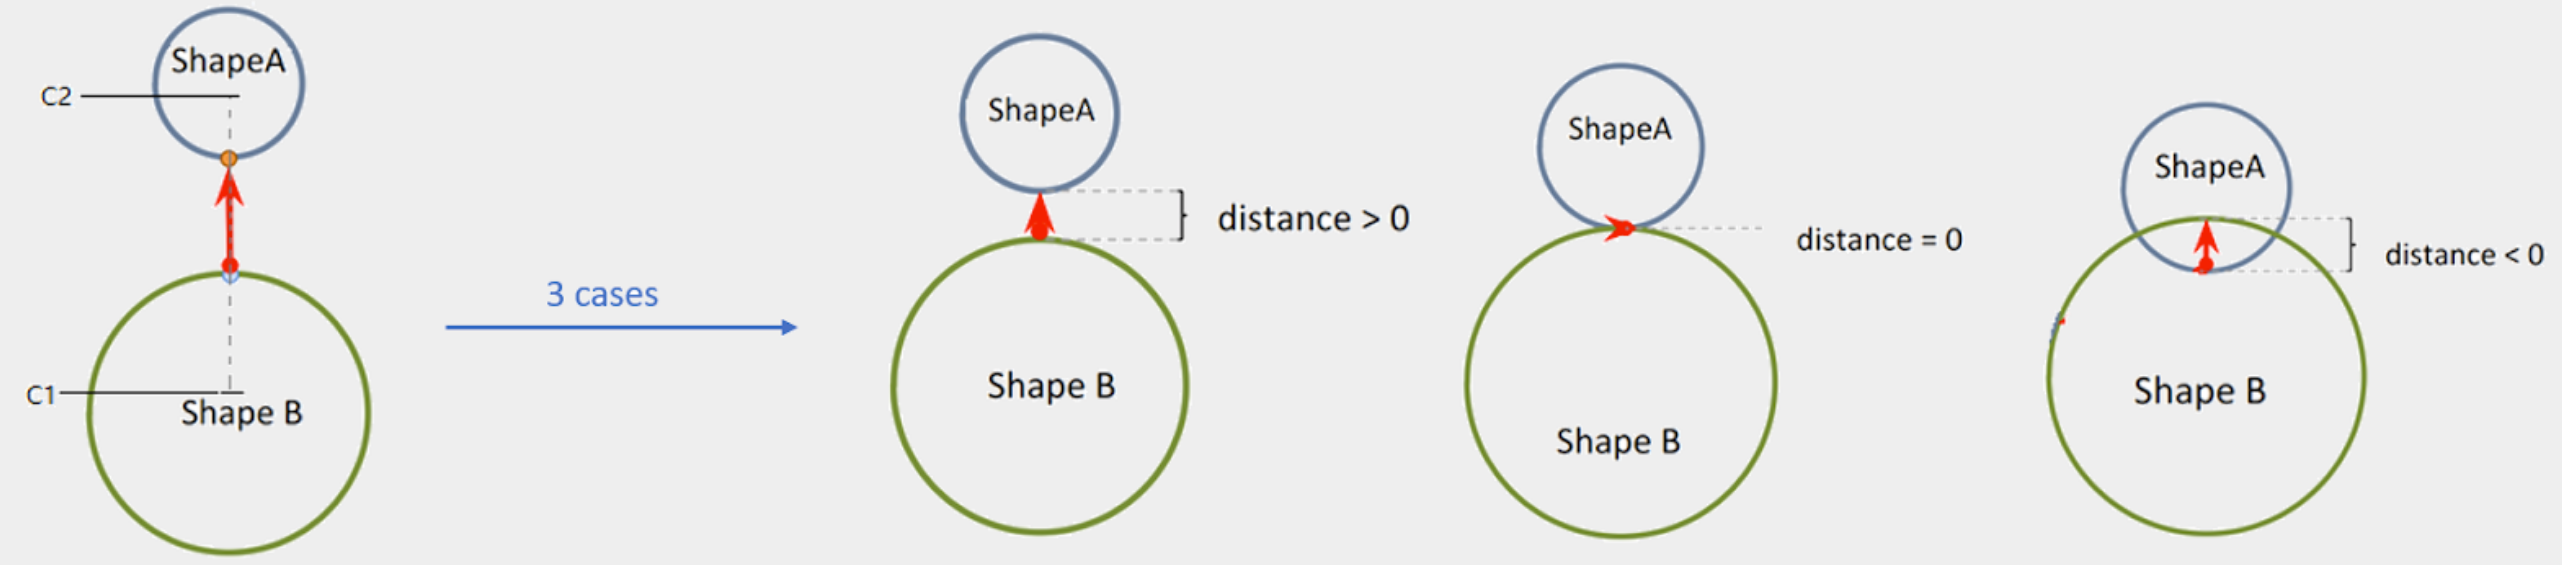
\includegraphics[scale=0.23]{images/sphere_sphere.png}
    \caption{Calculation of distance between two spheres}
    \label{fig:sphere_sphere}
\end{figure}

2) Distance between sphere and cylinder:
We calculate the distance between the sphere and a cylinder using below equation and the same is shown in the Figure \ref{fig:spherecapsule}.
\begin{equation}
	Closest point = X = 	\begin{cases}
        x = x_1 + \lambda(x_2 - x_1) \\
        y = y_1 + \lambda(y_2 - y_1) \\
        z = z_1 + \lambda(z_2 - z_1) 
    \end{cases}
    \label{eq:cpcyl}
\end{equation}

\begin{equation}
	\lambda = \frac{(c-m_1).(m_2-m_1)}{La^2}
\end{equation}

\begin{equation}
	Distance = |X-C| - (r_a + r_s)
\end{equation}

\begin{figure}[H]
    \centering
    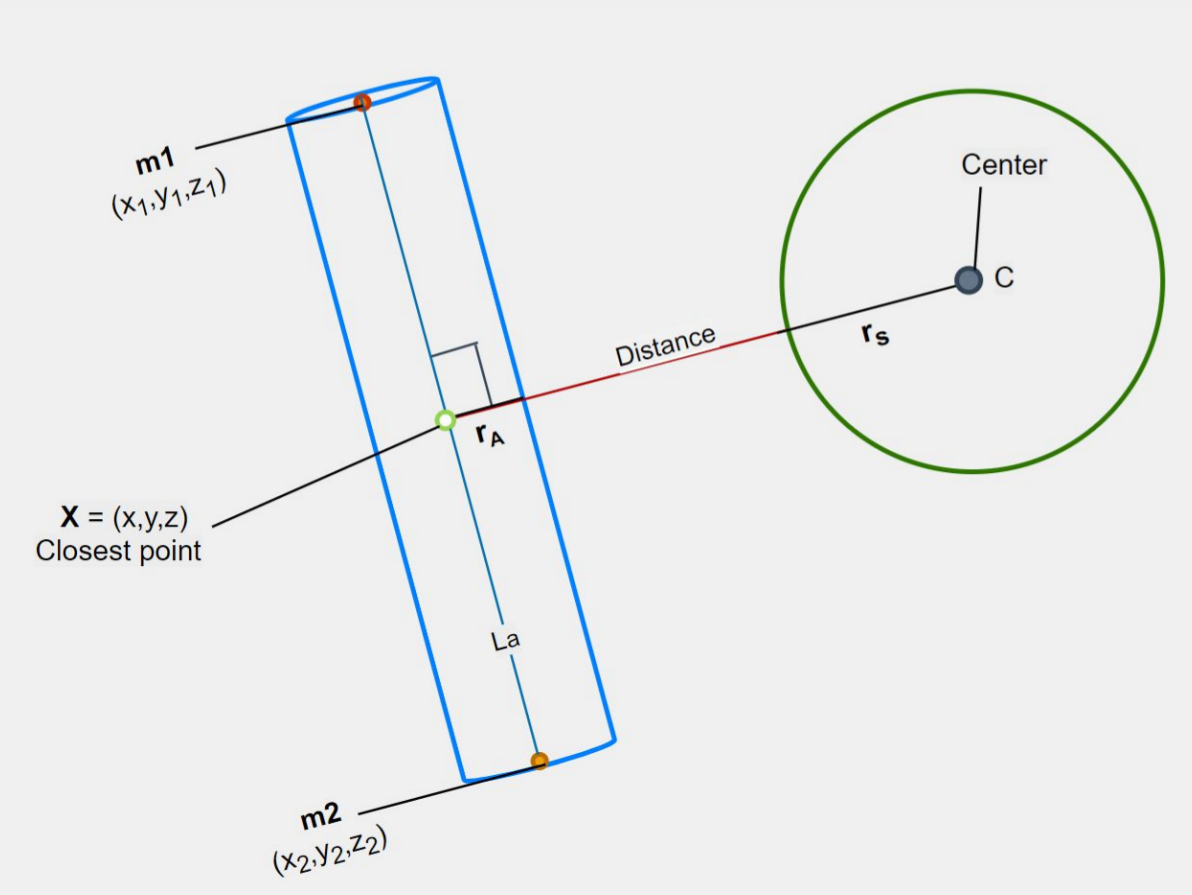
\includegraphics[scale=0.3]{images/sphere_capsule.png}
    \caption{Calculation of distance between a sphere and a cylinder}
    \label{fig:spherecapsule}
\end{figure}

3) Distance between two cylinders:
We compute the distance between the two cylinders based on the following four cases:
\begin{enumerate}
	\item m1 and m2 can be perpendicularly projected on to La.
	\item m1 and m2 cannot be perpendicularly projected on to La.
	\item Only m2 can be perpendicularly projected on to La.
	\item Only m1 can be perpendicularly projected on to La.
\end{enumerate}
Here, m1 and m2 refers to the starting point and end point of the symmetrical axis of shorter cylinder, La is the symmetrical axis of the longer cylinder. This is shown in Figure \ref{fig:capsule_capsule}.
\begin{figure}[H]
    \centering
    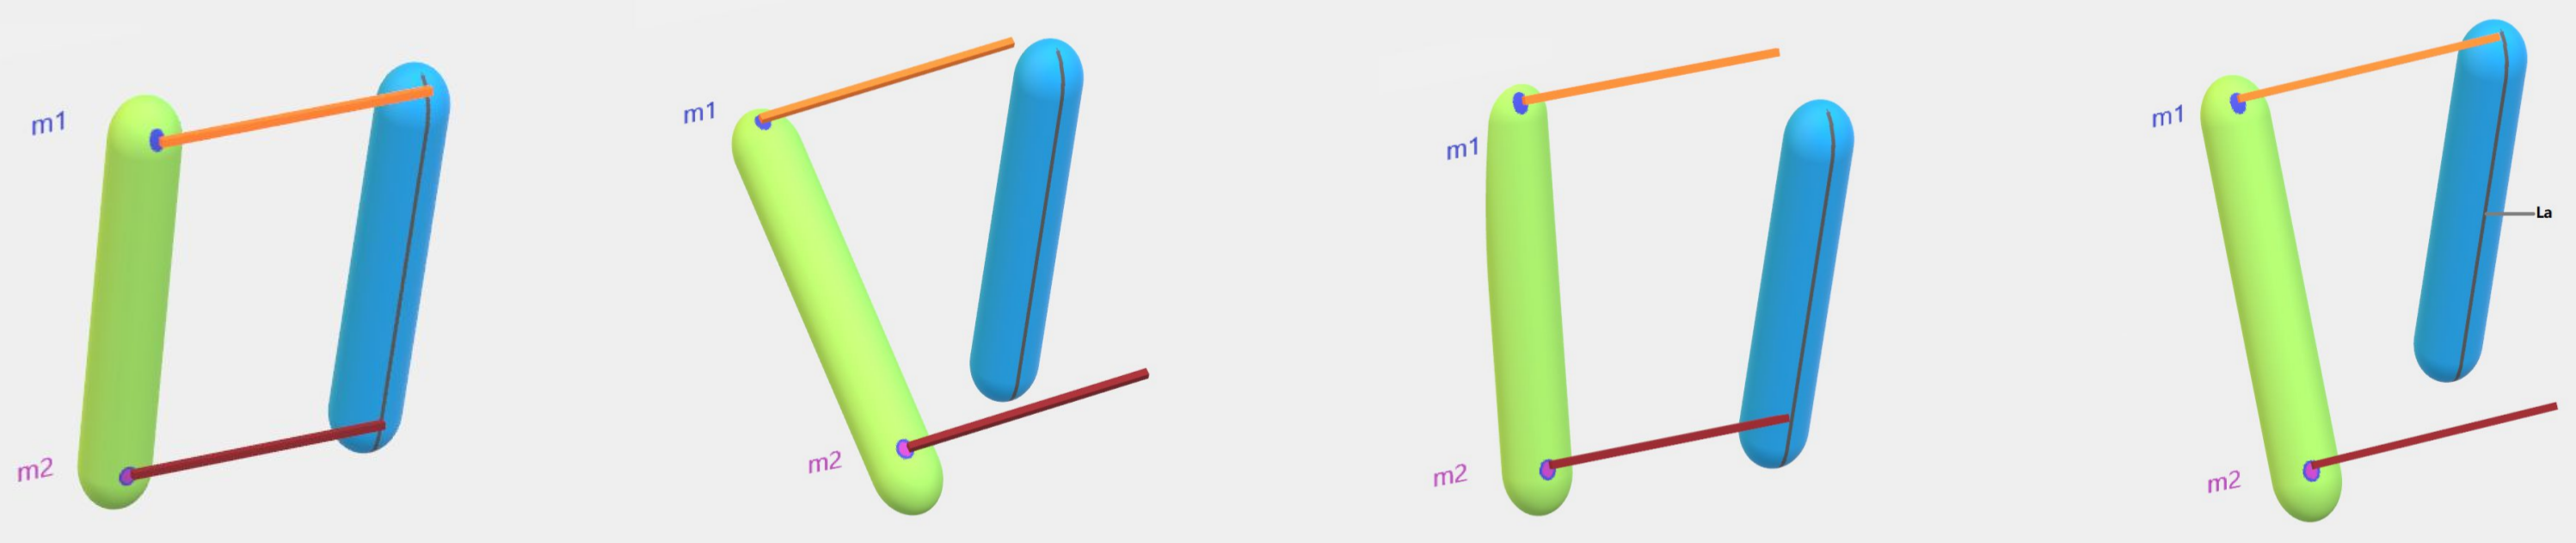
\includegraphics[scale=0.21]{images/capsule_capsule.png}
    \caption{Calculation of distance between two cylinders}
    \label{fig:capsule_capsule}
\end{figure}

4) Box configuration and closest point on the box:
As an extension to the previous work, here we have modeled the robot base as a 3D box or of cuboid shape. This box is considered as Axis Aligned Bounding Box (AABB) \cite{3ddet}, it means that the AABB doesn't have to have equal length, width, and height, but one condition here is that once it is configured the box should not be rotated. These AABBs are pivotal towards spatial partitioning. An example visualization is provided in Figure \ref{fig:aabb}. These boxes can be stored in two ways, first is to store the leftmost and rightmost corners and the second way is to store the center point of the box and a vector representing how far it extends in each x, y, z directions.

\begin{figure}[H]
    \centering
    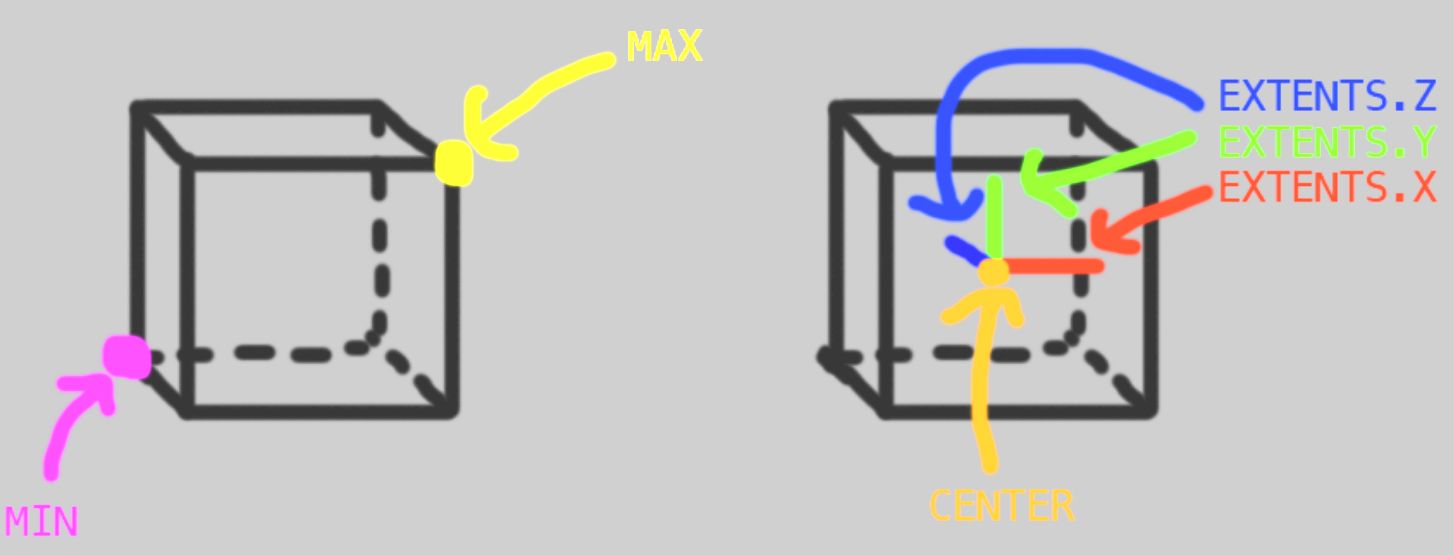
\includegraphics[scale=0.3]{images/aabb.png}
    \caption{Representation of AABB, image referenced from \cite{3ddet}}
    \label{fig:aabb}
\end{figure}

Initially we check if the given point is inside or on the box by comparing it to the position of leftmost corner (min) and rightmost corner (max). Since box has many edges and sides, we do have to figure out the closest point on the box that is closest to the obstacle. The algorithm to determine the closest point shows that the point will be clamped to AABB, that is we check if the point is outside the box and then compare the position of point with respect to min and max of the AABB and clamp the point to the nearest edge based on this comparison. If the point is inside the box, then the algorithm just returns the position of the point itself.

5) Distance between box and sphere:
To find the distance between the box and the sphere, first we have to consider the distance between the center of the sphere and the closest point on AABB. To find out the closest point of AABB we consider the sphere center to be the point of consideration. Once we have the closest point on box, we calculate the distance by using Equation \ref{eq:boxsp}. If this distance is less than the radius of the sphere, then we say that the box and sphere are intersecting \cite{3ddet}.

\begin{equation}
	Distance = Sphere.Position - ClosestPoint
	\label{eq:boxsp}
\end{equation}

6) Distance between box and cylinder:
A most widely implemented algorithm for collision detection in most physics engine used for game developments is GJK \cite{GJK}, this algorithm is based on creating convex hulls from two colliding convex geometry shapes by using minkowski sums \cite{min} that is by finding all difference of all the points on one object surface to the other.

We have minimized the implementation for our use case with two different complexities, one by considering only all the corner points and face centers of the box and the other by using all the edges of the box to calculate distance between the box and the other objects to avoid collision. This is visualized in Figure \ref{fig:bc2}.

\begin{figure}[H]
    \centering
    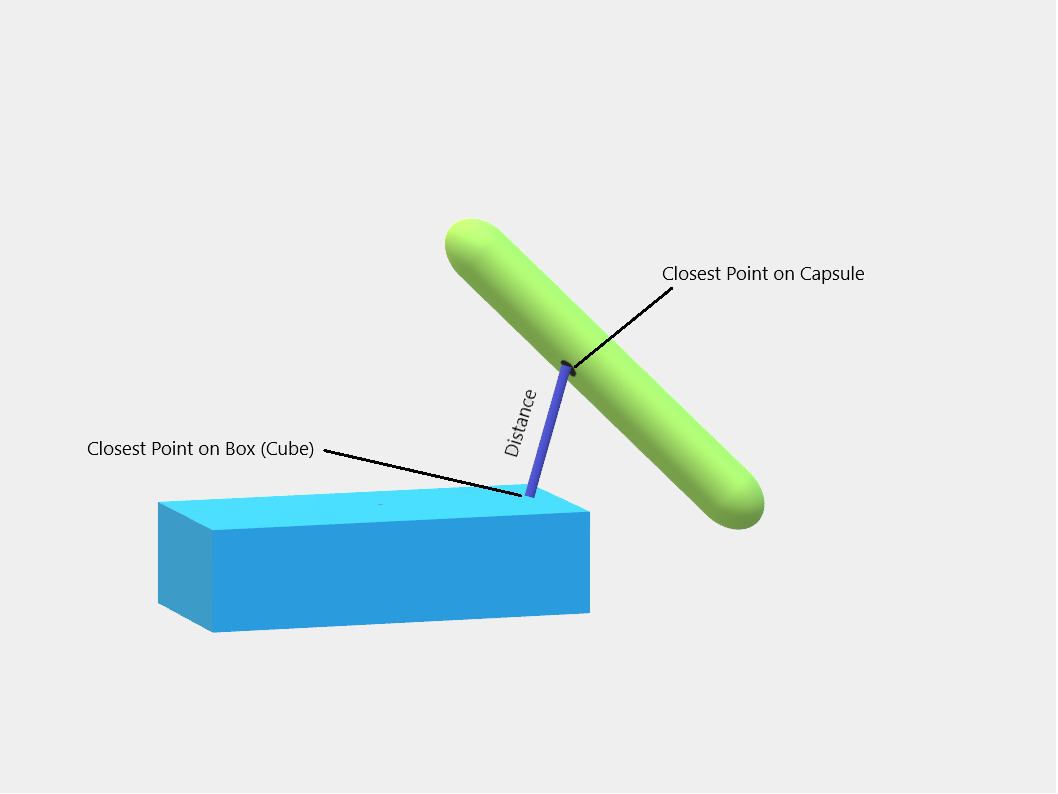
\includegraphics[width=0.7\linewidth, height=0.4\linewidth]{images/box_capsule.jpeg}
    \caption{Calculation of distance between a box and a cylinder}
    \label{fig:bc1}
\end{figure}

\begin{figure}[H]
    \centering
    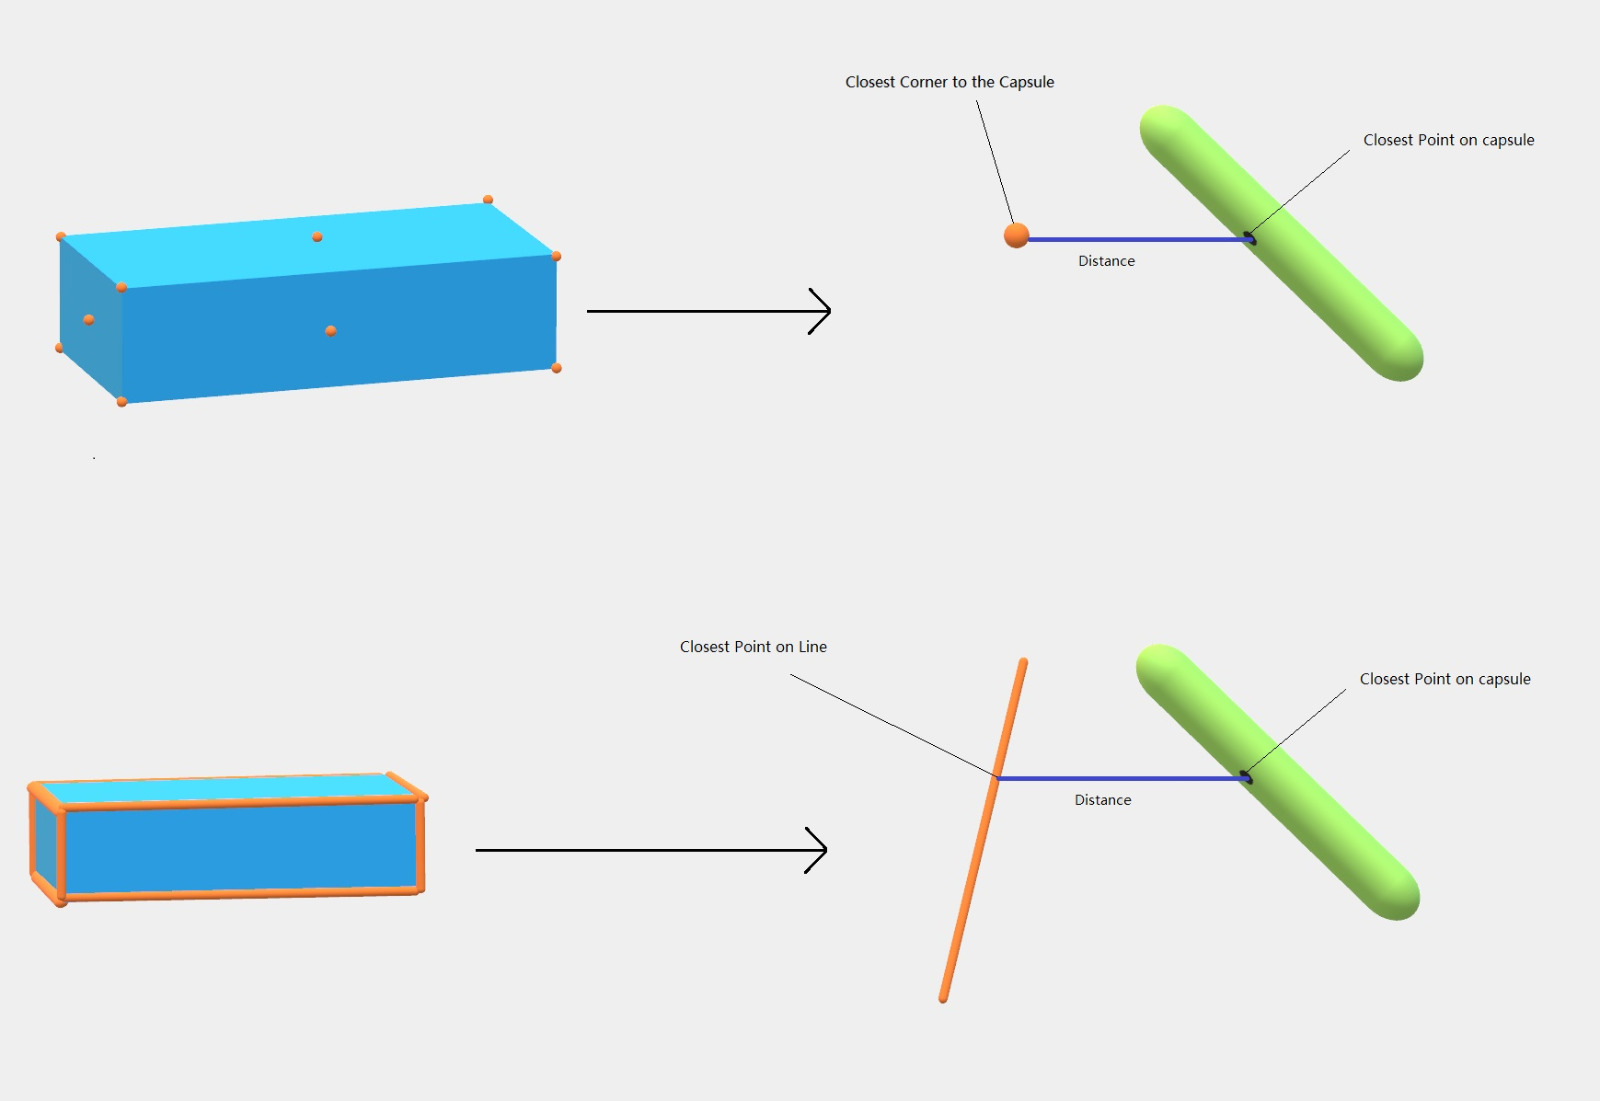
\includegraphics[width=0.7\linewidth, height=0.4\linewidth]{images/box_capsule1.jpeg}
    \caption{Determining the closest point on the AABB.}
    \label{fig:bc2}
\end{figure}

To find the distance between the box and the cylinder, fist we have to determine the closest point on the cylinder or capsule using the Equation \ref{eq:cpcyl}. We then clamp this closest point on to the AABB to find the closest point on the box. Once we have the two closest points, we consider the closest point of the cylinder or capsule to be the center point of the sphere and continue with the calculations by using the Equation \ref{eq:boxsp}. If this distance is less than the radius of the sphere (that is considered from the closest point on the cylinder or capsule to the edge of cylinder or capsule), then we say that the box is colliding with the cylinder or sphere \cite{3ddet}. This is visualized in Figure \ref{fig:bc1}.
\subsection{Potential field calculations}
In previous work, to avoid and monitor the collision between the robotic arms and the obstacles, the algorithm from \cite{Hoffmann} is implemented. This algorithm is based on the dynamic movement primitives (DMP) and is used to generate the new trajectories and velocities in real-time as given in below equations,
\begin{equation} \label{eq:1}
	\dot{v} = K ( g - x ) - D v - K (g - x_0) s + K f(s) + p(x, v)
\end{equation}
Where $g$ is goal position, $x$ is current position, $x_0$ is starting position, $v$ is current velocity, $s$ is phase variable, $D$ is damping constant, and $K$ is spring constant. The term $p(x,v)$ refers to the potential field generated by the obstacles which in turn helps in avoiding obstacles.

This potential field is calculated by determining the steering angle (Figure \ref{steering_image}) between the velocity vector and the vector from the obstacle to the end effector as shown in \ref{eq:2}. This steering angle provides information on the sharpness of the steering of end effector from obstacle. Using this angle, the potential field is calculated as given in Equation \ref{eq:3}.

\begin{figure}[H]
	\centering
	\scalebox{0.55}{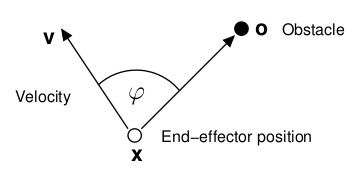
\includegraphics{images/steering_angle.png}}
	\caption{Graphical representation of steering angle \cite{Hoffmann}}
	\label{steering_image}
\end{figure}

\begin{equation} \label{eq:2}
	\varphi = cos^{-1}\Bigg( \frac{(o-v)^T v}{\|o-x\| \cdot \|v\|}\Bigg)
\end{equation}
\begin{equation} \label{eq:3}
	p(x, v) = \gamma \sum_i R_i v \varphi_i exp(-\beta \varphi_i) 
\end{equation}

Where $\gamma$ and $\beta$ are tune-able constants, and R is a rotation matrix which rotates by the axis $r = (o-x) \times v $ with an angle of rotation of $\pi/2$. This rotation matrix can be calculated using the following approach described in \cite{rodrigues}. The final potential field is the sum of the potential fields generated by all the obstacles. The final equation converges towards the goal avoiding the obstacles as given below.

\begin{equation}
\dot{v} = K ( g - x ) - D v + p(x, v)
\end{equation}

\begin{figure*}[t]
	\centering
	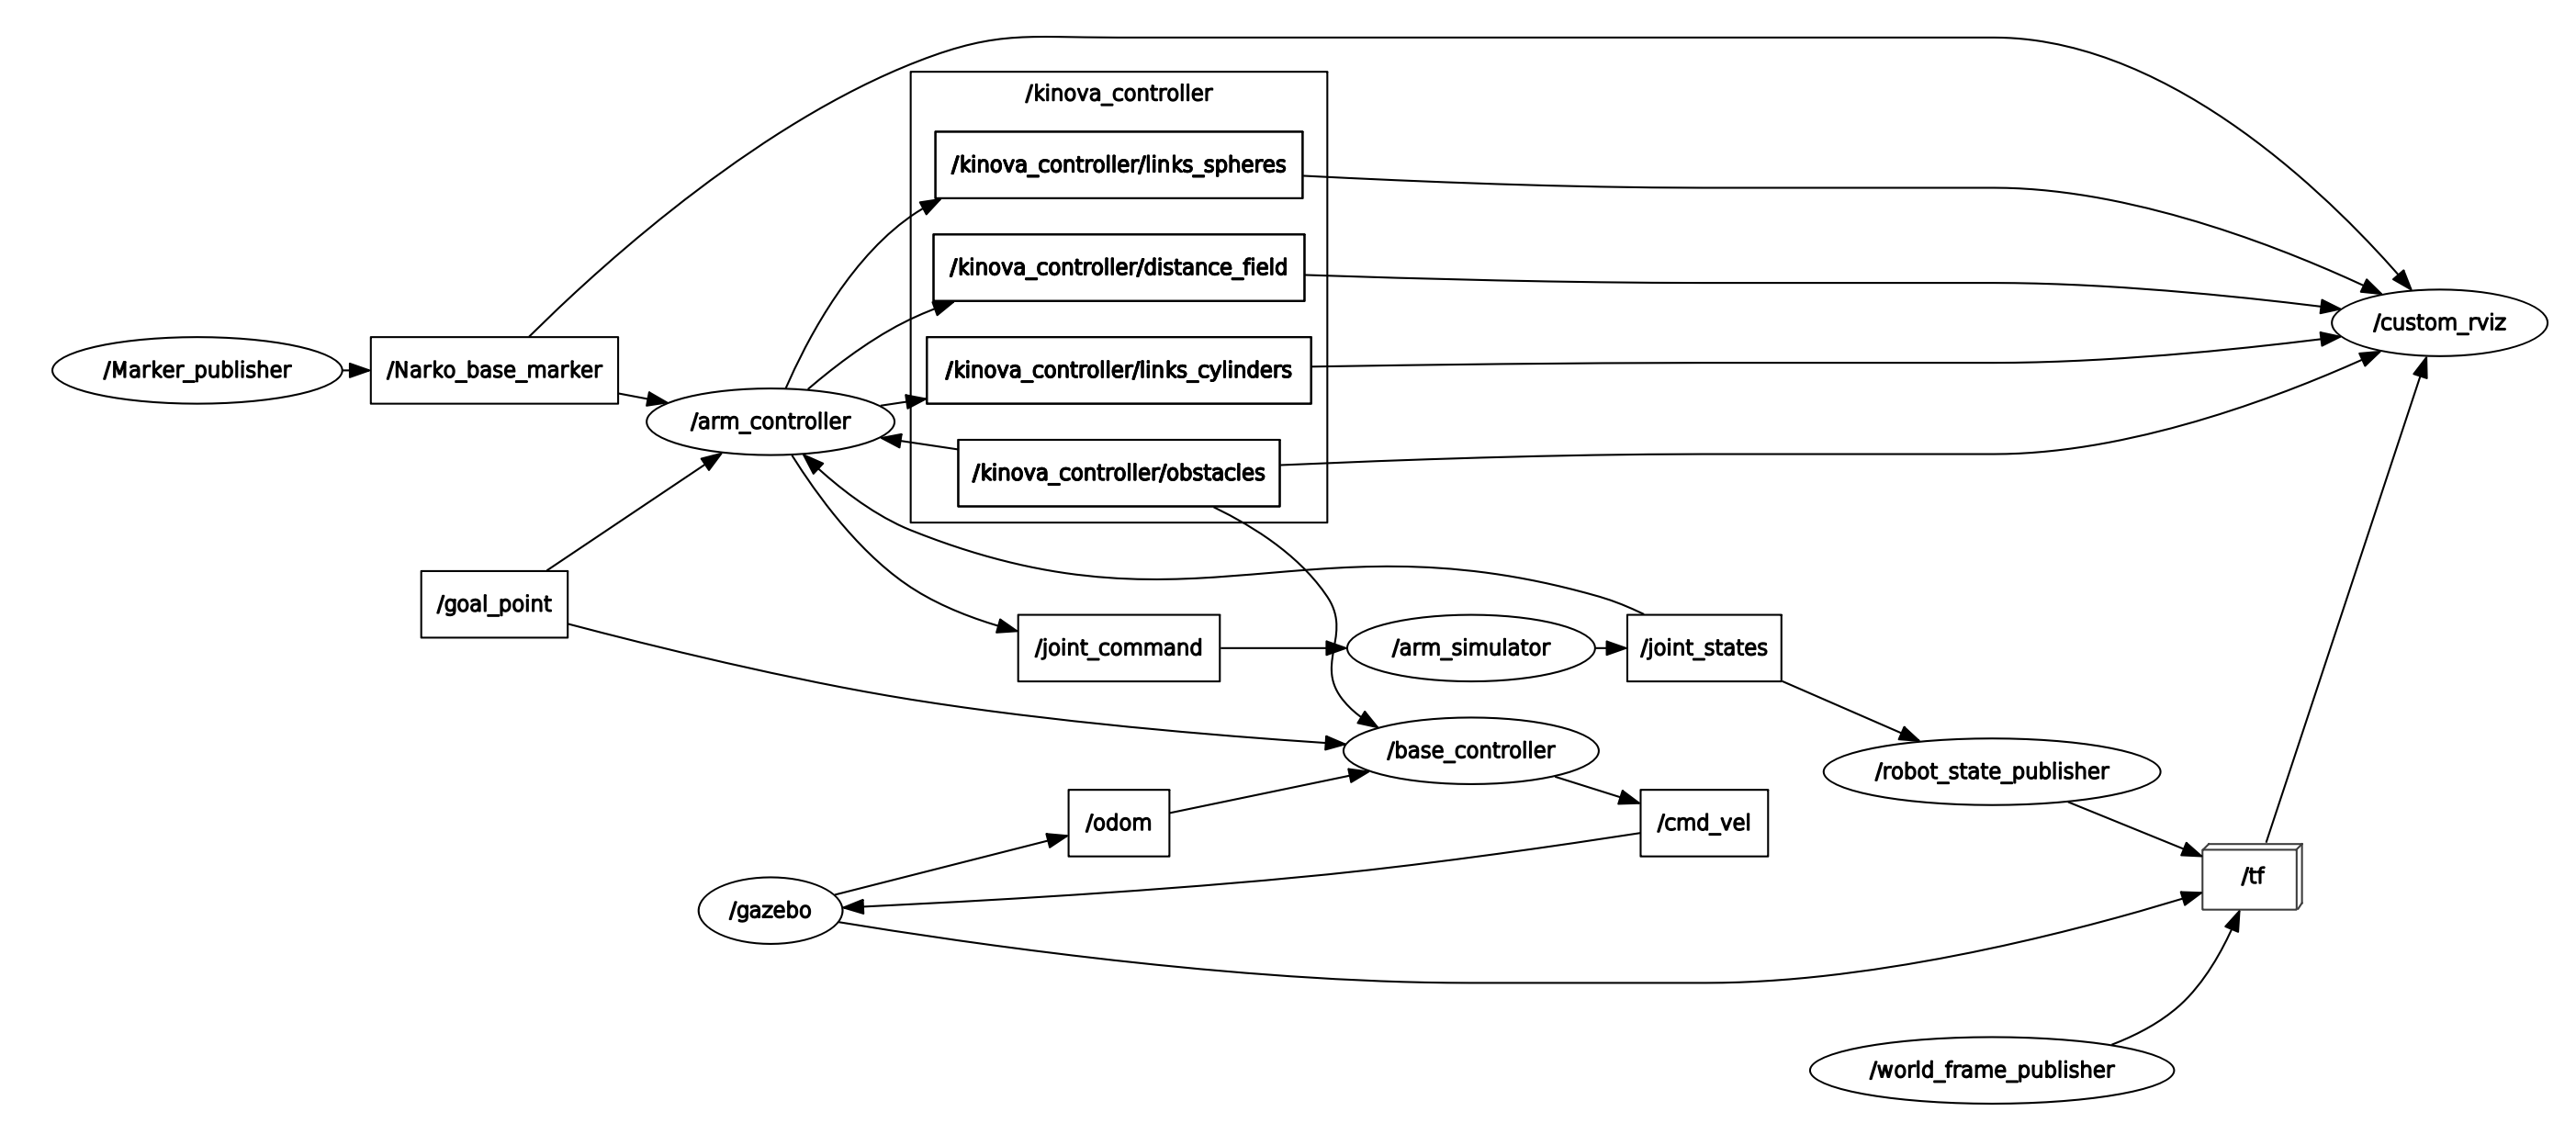
\includegraphics[width=1.0\linewidth, height=0.2\linewidth]{images/ros_graph.png}
	\caption{ROS node graph showing the communication flow between the subcomponents of the package.}
	\label{fig:rosgraph_single}
\end{figure*}

\subsection{Collision monitoring library}
This work is an extension of the the previous work. Here along with the robot arms from previous implementation, we also model the robot base such that the arms do not collide with the base while performing some actions. Along with this extension, we also implemented the base control algorithm which actively helps in monitoring and avoiding collision between the robot base and other obstacles in the workspace.

In order to monitor the distance between the links of the robot arm, obstacles, robot base in the workspace, the links are modeled as the cylinders, end effectors are modeled as spheres, and the robot base is modeled as the 3D box. This type of modeling helps in easier calculations of distance between two primitives which results in monitoring of the self collision of the arms and base. This kind of modeling helps in easier calculation of potential fields, determining the nearest points or closest points on the primitives and obstacles that helps in calculating the distances, which in turn results in real-time collision monitoring and avoidance.

\subsection{Controller} 
In this work, we follow the same architecture for the base controller as the previous work. Since we perform the collision monitoring and avoidance between the arms and the base, both the arm controller and the base controller are necessary. As per the previous work, the arm controller is controlled via a control loop which executes at a specific rate and provides the geometric locations which updates the velocity of the arms in real-time. Similarly, the base controller is also controlled via a control loop which executes at a specific rate and provides information on the geometric location of the mobile base and the velocity updates. This real-time information on the positions of arm and the base helps in quicker calculation of distances and helps in collision avoidance and monitoring with self and other obstacles in the workspace.
 
\section{Implementation}
In this work, we built the extension and the base controller implementation on the ROS platform, and tested with ROS kinetic and melodic versions. There are various libraries such as Kinova Kortex library \cite{kortex}, this library provides various high and low level control APIs for handling the robotic manipulators, Kinova\_arm package that provides the design details, and implementation details for the robotic arms. Along with these libraries, in this work we make use of narko\_description for creating the robot mobile base and connect the arms and the base. The final standalone library does not depend on any ROS components, and these ROS components are used only for testing and simulation of the collision avoidance and monitoring library.

The standalone library for collision monitoring and avoidance is purely developed using the C++ programming language, we make use of ROS and python for testing, simulation, and publishing of the robot base nodes. Similar to the previous work, the package is is divided into three subcomponents, the controller for base and arms, simulator and visualization. From previous work we have the arm controller implementation based on \cite{Hoffmann}, and as an addition to this, we extended by adding the robot base as a box primitive to monitor and avoid the collision of arms with robot base. Addition to this, we implemented a base controller that helps in avoiding and monitoring the collisions with obstacles in the workspace. To visualize this, we have implemented a differential drive setup for movement and visualization of robot.

Similar to previous implementation, here we have implemented the collision avoidance part of the library in a control loop, that executes continuously to obtain the shortest distance vectors from the robot base and the obstacles. This shortest distance is then used for calculating the potential field along with the current velocity resulting in a new velocity and path for avoiding the collision and maneuvering towards goal position. This new velocity is then provided to the NarkinBase class for mapping the new velocity from Cartesian space to the robot base space.

The simulation software takes the new velocity, obstacle position and information on the potential field and generates a new position for the robot, and this new position is then passed on to the base controller such that it avoids the collision with obstacle and moves towards the goal position. This works in a loop until the robot reaches the goal position. 

A basic ROS node graph showing the communication flow between the subcomponents of the standalone package is shown in Figure \ref{fig:rosgraph_single}. Here we use the interfaces to add the obstacle to the workspace, and also to provide the goal position. For visualization, we make use of the in-built robot\_state\_publisher node and Rviz.

\section{Evaluation}
In this section, we will discuss about experimental setup and evaluation of the implemented library.

\subsection{Collision Monitoring}
As an extension of the previous work, the computations behind the control algorithm is purely based on mathematics and hence the library do not have any practical measure of accuracy. To verify the computations and working of the library, we make use of ROS for creating an working environment which helps in simulation of working robot which is controlled using the implemented control algorithm. To have the consistency and the similar speed compared to previous work, this extension work is also implemented using C++. The performance test of this library was performed on Ubuntu 16.04 and Ubuntu 18.04 machines, including Ubuntu virtual machine.

For evaluation of this work, we make use of ROS simulations, where the kinova interfacer provides an interface for interacting with the robot workspace for adding the obstacles, and providing goal points. Here we evaluate the working of the collision monitoring and avoidance between the robot arm and the robot base, along with this we also evaluate the collision avoidance between the obstacles in the workspace and the robot base. To achieve the similar speed as previous work, for testing purpose we have made use of the same values for k, d, gamma, and delta that are used in the calculations of new velocity, potential field, and steering angle.

For the visualization of the robot base we have used narko description which provides the robot description in the for of urdf fines and meshes, and we have used kinova\_arm package which provides the robot description of arm in the form of urdf file for arm visualization. Each link in the arm is modeled as capsules or cylinders and the robot base as 3D box or cuboid. The same is visualized in Figure \ref{fig:robot}.

\begin{figure}[H]
	\centering
	\scalebox{0.25}{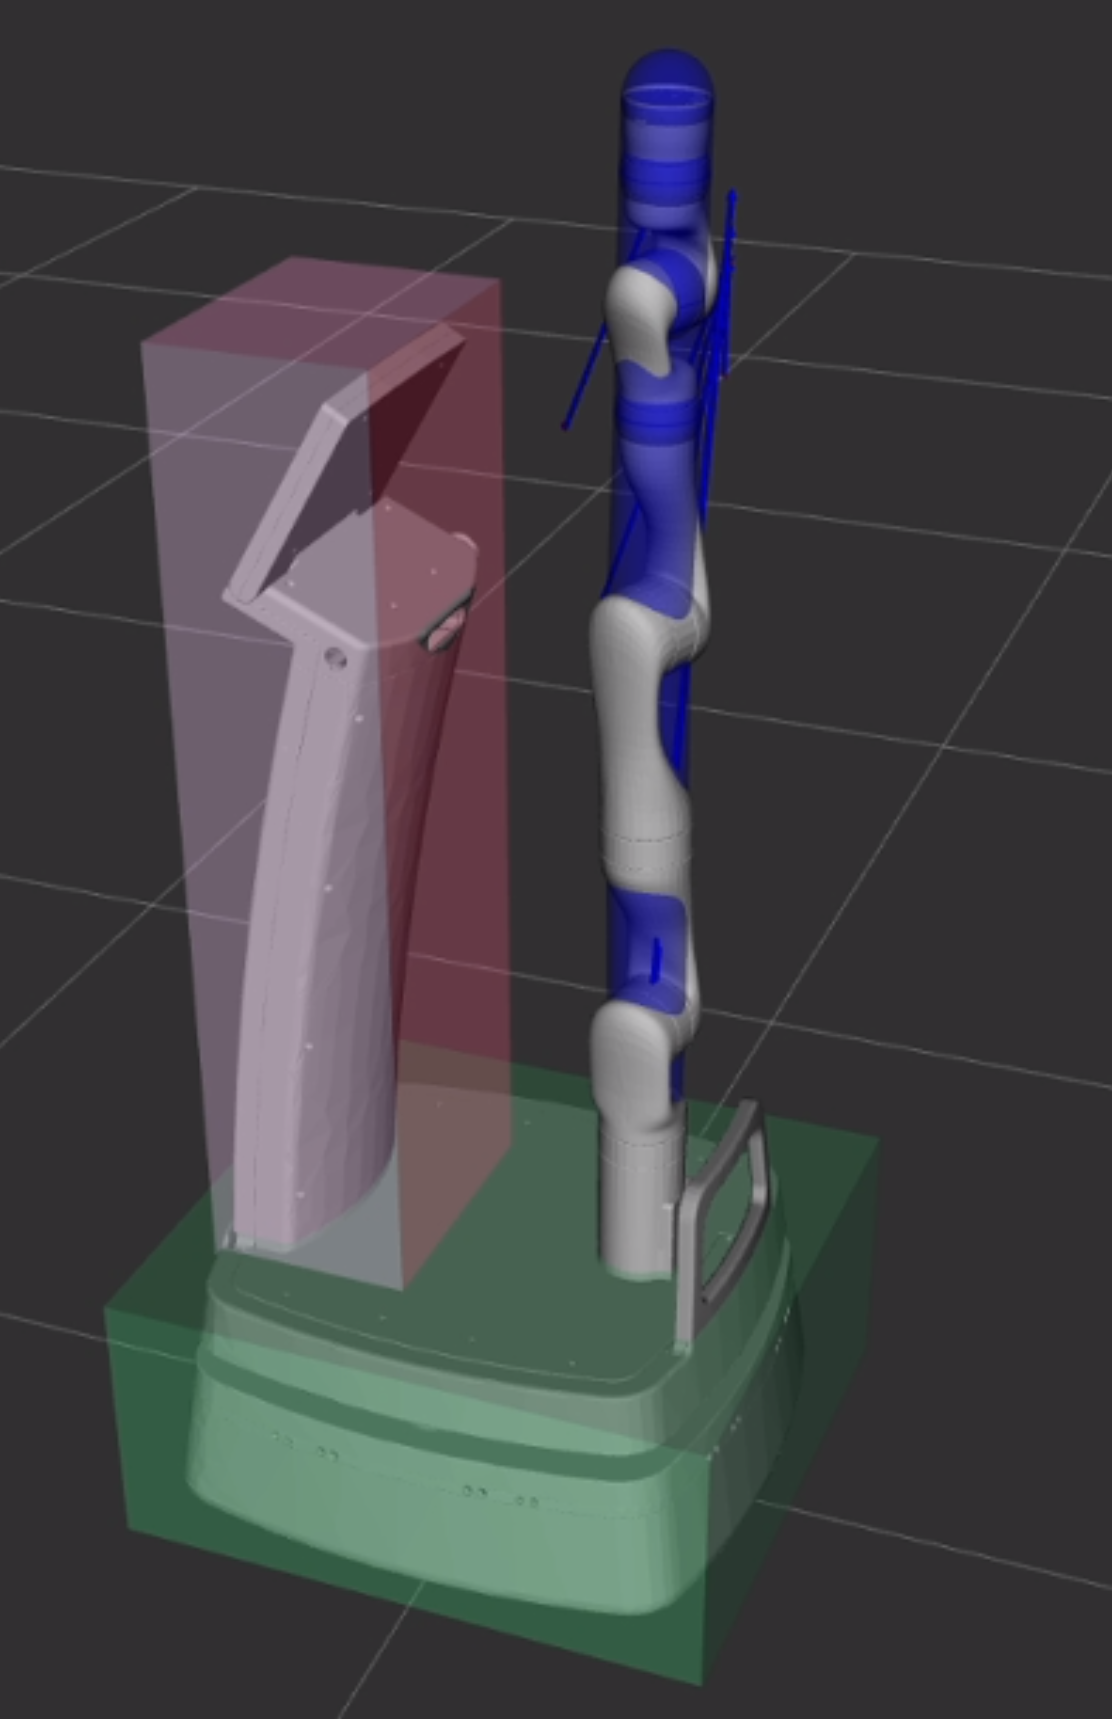
\includegraphics{images/robot.png}}
	\caption{Visualization of robot along with the modeled primitives.}
	\label{fig:robot}
\end{figure}

\subsubsection{Collision avoidance between arm and robot body}
In this work, to avoid the self collision between the arm and the body, we have modeled the robot base as to be an obstacle with respect to the arm controller. The control algorithm treats this cuboid or the robot base as an obstacle and when ever the arm moves near to the body, the control algorithm generates the signal for active monitoring to avoid the collision. This is shown in Figure \ref{fig:robot1}.

\begin{figure}[H]
	\centering
	\label{potential}
	\begin{subfigure}[t]{0.20\textwidth}
		\centering
		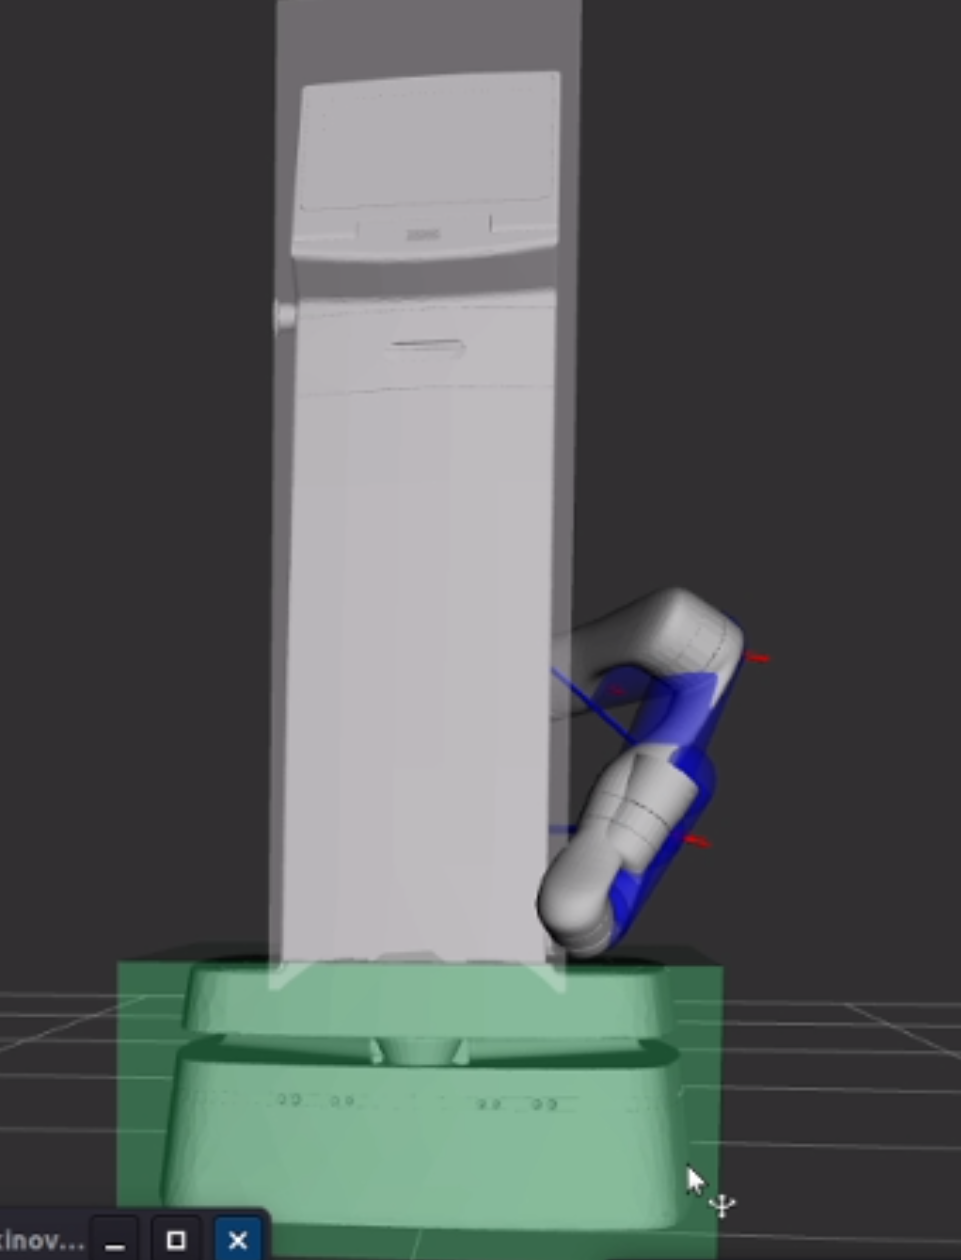
\includegraphics[scale=0.273]{images/robot1.png}
		
	\end{subfigure}%
	~ 
	\begin{subfigure}[t]{0.20\textwidth}
		\centering
		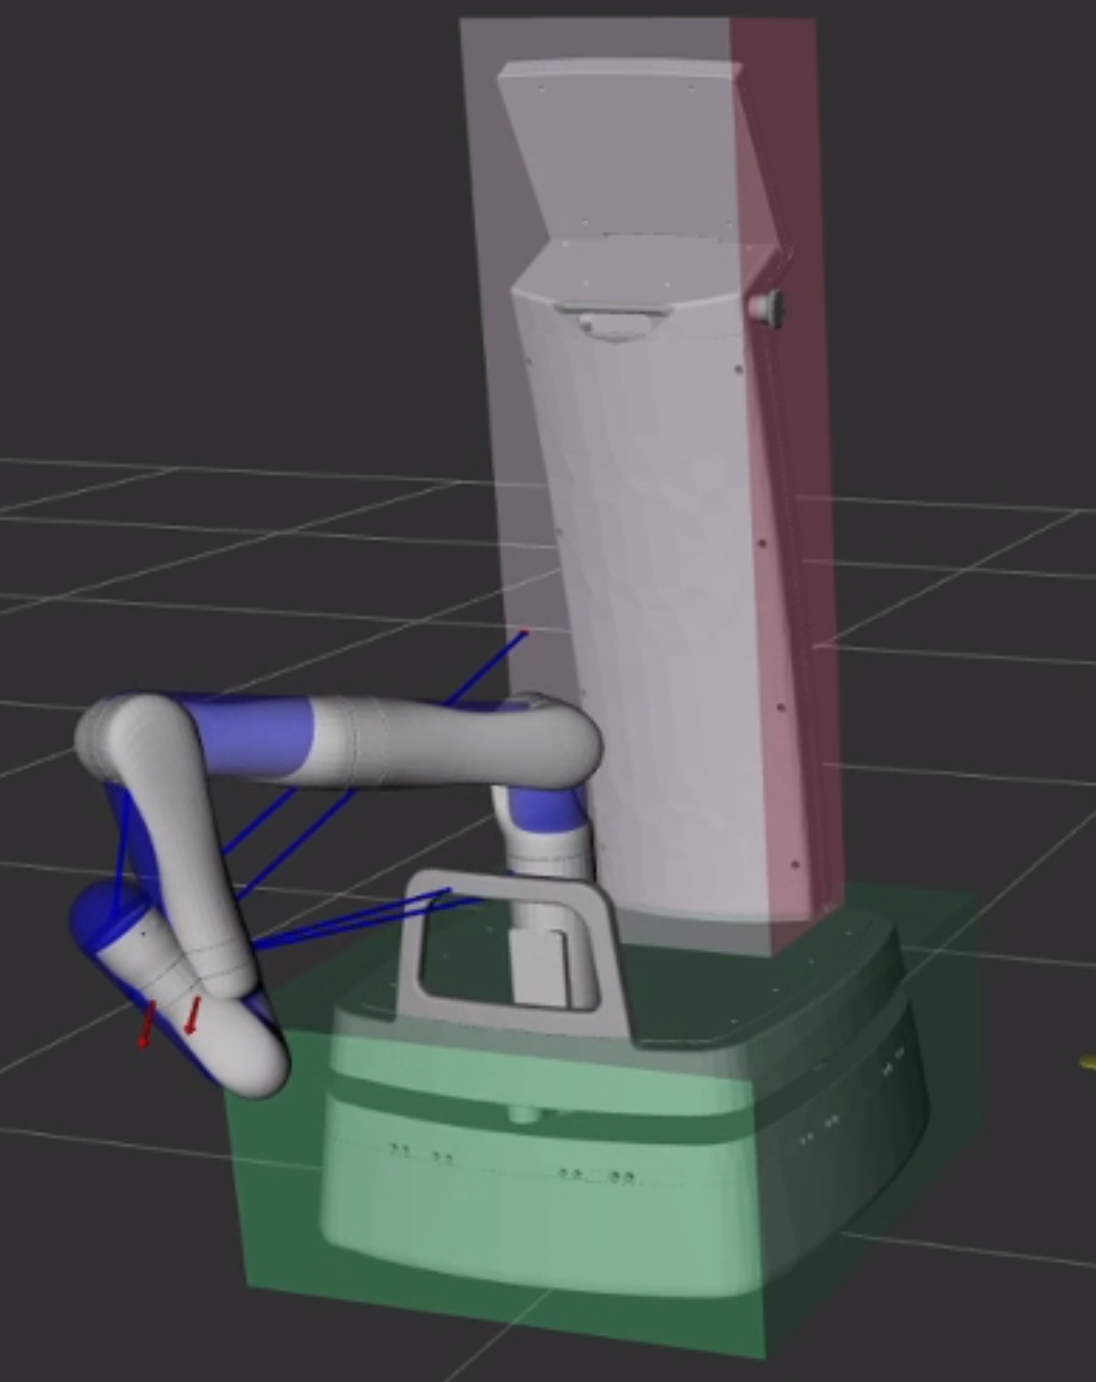
\includegraphics[scale=0.25]{images/robot2.png}
		
	\end{subfigure}
	\caption{Active monitoring of self collision.}
	\label{fig:robot1}
\end{figure}

The control algorithm actively monitors the movement of the robot arm even when they are stand still. As seen in the left image of the Figure \ref{fig:robot1}, when the robot arm moves near to the robot body, the control algorithm generates signals by making use of the potential field and the new velocities to avoid colliding with the body, this is shown using the red arrow in the simulation. Similarly, when the robot arm moves near the robot base, the red arrows from the active monitoring are visible in the simulation.


\subsubsection{Collision avoidance between robot and the obstacles}
Along with the monitoring of the self collision, we have also implemented the base control algorithm that actively monitors and avoids collision with obstacles in the workspace. For simulation of the robot movement, we have implemented a two wheel differential drive robot using the narko description and for movement of the robot we have implemented a PID controller. Here we have implemented the algorithm for calculation of the distance between the base and the obstacles. The initial distance between the obstacle and the robot base is visualized in the Figure \ref{fig:robot5}.

\begin{figure}[H]
	\centering
	\scalebox{0.4}{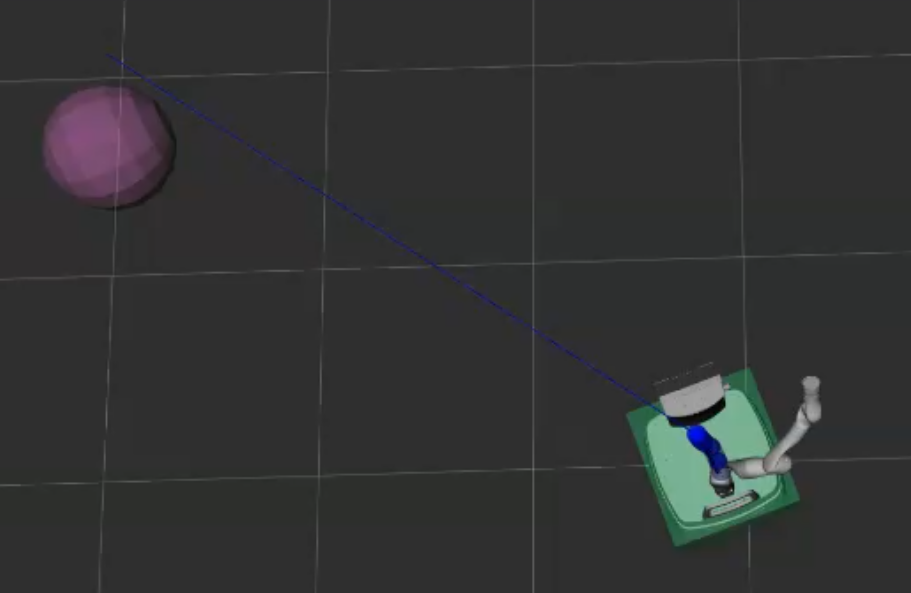
\includegraphics{images/robot5.png}}
	\caption{Visualization of initial distance between robot and obstacle.}
	\label{fig:robot5}
\end{figure}

During testing of the base controller algorithm for avoiding collision with obstacles, we noticed that due to some calculation errors with respect to the translation of obstacle pose into robot base space, the algorithm for collision avoidance does not work properly and proper conversion mechanism and optimization techniques needs to be implemented to solve the problem. The result of this calculation glitches is visualized in Figure \ref{fig:robot6}. Currently, the object pose is translated on to the arm space and the initial position of the obstacle varies as and when the robot moves. Due to time constraints, this was not corrected in this implementation.

\begin{figure}[H]
	\centering
	\scalebox{0.4}{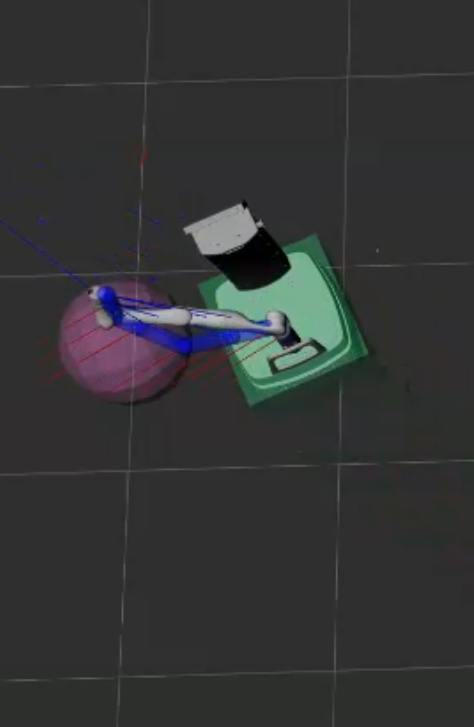
\includegraphics{images/robot6.png}}
	\caption{Visualization of wrong movement generation due to calculation errors.}
	\label{fig:robot6}
\end{figure}



\section{Use cases}

\subsection{Arm}
Since this work is an extension of previous work, all the features that were implemented related to the arms still functions and can be used to create and experiment with multiple number of arms. Considering single arm, the arm controller looks and helps in avoiding and monitoring the collision of end-effector with the obstacles in the workspace. Considering dual arms, the links and joints of the arms are represented as obstacles, hence both arms do not collide with each other and also they do not collide with the obstacles. Any number of obstacles can be added to the workspace using the interfacer provided in the library. Similarly, the library is capable of handling more than two arms and they have to be configured before execution of the library.

\subsection{Base}
In this work, the robot base is modeled as a 3D box or can be referred to as a cuboid. This cuboid is treated as an obstacle from the arm controller point of view and this helps in avoiding and monitoring of self collision between arm and the base. This cuboid representation acts as a generic representation since most of the robot's base is either of a cuboid shape or of cylindrical shape and can be enclosed using a cuboid. Along with this, the base controller implementation (currently buggy) looks out for obstacles in the workspace and actively monitors and avoids collision.

\section{Conclusion}
This work is an extension of \cite{sdpss20}, where the existing library is extended to perform collision monitoring and avoidance of robot arms with robot base. To achieve this, we explored various modeling techniques and algorithms of which \cite{GJK} provides promising performance with respect to distance calculation between objects, but implementation and testing of this algorithm requires more complex computations and hence we chose to model the robot base as Axis Aligned Bounding Boxes (AABB) \cite{3ddet} which are easier to store and computations are simpler as discussed in the previous sections. This AABB modeling approach also provides easier and simpler ways for performing unit tests.

As an extension to the existing library, we modeled the robot base as an obstacle with respect to the arm controller such that it helps in avoiding and monitoring self collision. To this extent we were successful in achieving the active monitoring of the self collision. Although this implementation works as expected, there is always a room for optimization.

Along with this we also implemented a base controller which actively monitors the collision between the obstacles and the robot base. We implemented a PID controller and two wheel differential drive robot using the narko description for movement control of the robot. We were successful in calculating the distance between the obstacles and the robot base. But due to error in calculating the translation of new positions and velocities from one space to other, the active monitoring does not work as expected and due to time constraints, we were not able to fix it.

As future work, we would like to stress more on the optimization part of the self collision and to implement more effective control algorithm for the robot base.

\addtolength{\textheight}{-12cm}   % This command serves to balance the column lengths
                                  % on the last page of the document manually. It shortens
                                  % the textheight of the last page by a suitable amount.
                                  % This command does not take effect until the next page
                                  % so it should come on the page before the last. Make
                                  % sure that you do not shorten the textheight too much.

%%%%%%%%%%%%%%%%%%%%%%%%%%%%%%%%%%%%%%%%%%%%%%%%%%%%%%%%%%%%%%%%%%%%%%%%%%%%%%%%



%%%%%%%%%%%%%%%%%%%%%%%%%%%%%%%%%%%%%%%%%%%%%%%%%%%%%%%%%%%%%%%%%%%%%%%%%%%%%%%%
\section*{Appendix}
The code for the collision monitoring library is accessible at the following link: \url{https://github.com/Sreeni1204/sdp\_ws20\_collision\_monitoring\_for\_mobile\_manipulators}

%%%%%%%%%%%%%%%%%%%%%%%%%%%%%%%%%%%%%%%%%%%%%%%%%%%%%%%%%%%%%%%%%%%%%%%%%%%%%%%%
\section*{Acknowledgements}
We would like to thank Djordje Vukcevic for his support and motivation throughout the course of this project.

%%%%%%%%%%%%%%%%%%%%%%%%%%%%%%%%%%%%%%%%%%%%%%%%%%%%%%%%%%%%%%%%%%%%%%%%%%%%%%%%


\begin{thebibliography}{10}
	
\bibitem{Khatib} O. Khatib, “Real-Time Obstacle Avoidance for Manipulators and Mobile Robots” The International Journal of Robotics Research, vol. 5, no. 1, pp. 90–98, Mar. 1986, doi: 10.1177/027836498600500106.
\bibitem{Hoffmann} H. Hoffmann, P. Pastor, D.-H. Park, and S. Schaal, “Biologically-inspired dynamical systems for movement generation: Automatic real-time goal adaptation and obstacle avoidance,” in 2009 IEEE International Conference on Robotics and Automation, Kobe, May 2009, pp. 2587–2592, doi: 10.1109/ROBOT.2009.5152423.
\bibitem{Fadalil} M. S. Fadali and A. Visioli, “Introduction to Digital Control,” in Digital Control Engineering, Elsevier, 2013, pp. 1–8.
\bibitem{Adee} S. Adee, “Dean Kamen’s ‘Luke Arm’ Prosthesis Readies for Clinical Trials - IEEE Spectrum,” IEEE Spectrum: Technology, Engineering, and Science News, Feb. 01, 2008. https://spectrum.ieee.org/biomedical/bionics/dean-kamens-luke-arm-prosthesis-readies-for-clinical-trials (accessed Jun. 25, 2020).
\bibitem{Janabi-Sharif} F. Janabi-Sharifi and D. Vinke, “Integration of the artificial potential field approach with simulated annealing for robot path planning,” in Proceedings of 8th IEEE International Symposium on Intelligent Control, Aug. 1993, pp. 536–541, doi: 10.1109/ISIC.1993.397640.
\bibitem{rodrigues}  Belongie, Serge. "Rodrigues' Rotation Formula." From MathWorld--A Wolfram Web Resource, created by Eric W. Weisstein. https://mathworld.wolfram.com/RodriguesRotationFormula.html 
\bibitem{kortex} Kinovarobotics/ros\_kortex. Kinova Robotics, 2020.
\bibitem{GJK} E. G. Gilbert, D. W. Johnson and S. S. Keerthi, "A fast procedure for computing the distance between complex objects in three-dimensional space," in IEEE Journal on Robotics and Automation, vol. 4, no. 2, pp. 193-203, April 1988, doi: 10.1109/56.2083.
\bibitem{3ddet} AABB · 3DCollisions - \url{https://gdbooks.gitbooks.io/3dcollisions/content/Chapter1/aabb.html}, Accessed on 03/07/2021
\bibitem{sdpss20} A. Gomez, S. Parra and B. Penfold, “Implementation of biologically-inspired dynamical systems for movement generation: automatic real-time goal adaptation and obstacle avoidance”, 2020.
\bibitem{min} Coulombe, A., and Lin, H.-C. (2020). High Precision Real Time Collision Detection. ArXiv Preprint ArXiv:2007.12045.
%\bibitem{Velliste} M. Velliste, S. Perel, M. C. Spalding, A. S. Whitford, and A. B. Schwartz, “Cortical control of a prosthetic arm for self-feeding,” Nature, vol. 453, no. 7198, Art. no. 7198, Jun. 2008, doi: 10.1038/nature06996.



\end{thebibliography}


\end{document}